\documentclass[11pt,letterpaper,titlepage,oneside]{book}
%\documentclass[10pt,letterpaper,titlepage,oneside,twocolumn]{book}
%\setlength{\columnsep}{distance}
\usepackage[english]{babel}
\usepackage[utf8x]{inputenc}
\usepackage{amsmath}
\usepackage{graphicx}
\usepackage{multicol}
\usepackage[parfill]{parskip}
\usepackage{anysize}
\usepackage{amssymb}
\usepackage{empheq,amsthm}
\usepackage[Lenny]{fncychap}
\usepackage{xcolor}
\usepackage{cancel}
\usepackage[justification=centering]{caption}
\usepackage{hyperref}

\newcommand{\degr}{\ensuremath{^\circ}}
\newcommand{\htab}{\hspace{0.5cm}}
\newcommand{\hhtab}{\htab\htab}
\newcommand{\where}{\htab\text{where }}
\newcommand{\andd}{\htab\text{and}\htab}

\newcommand{\kcol}[1]{\textcolor{blue}{#1}}
\newcommand{\mcol}[1]{\textcolor{red}{#1}}

\oddsidemargin 0.0in
\evensidemargin 0.0in 

%\setlength{\columnsep}{24pt}

\title{PHYS 232: Heat \& Waves \\ Waves Study Notes}
\author{Luke Zhou \\ McGill University}
\date{Winter 2013 \& Summer 2023}

\begin{document}
\maketitle
%\belowdisplayskip=0pt 
%\abovedisplayskip=5pt 

%\setlength{\abovedisplayskip}{0pt}
%\setlength{\belowdisplayskip}{0pt}
%\setlength{\abovedisplayshortskip}{0pt}
%\setlength{\belowdisplayshortskip}{0pt}

\frontmatter
\tableofcontents 

\mainmatter 
\chapter{Periodic Motion}
\section{Simple Harmonic Motion}
\begin{align*}
\shortintertext{Restoring forces for a displacement $x$:} 
F(x) &= -(k_1 + k_2x^2 + k_3x^3 + \cdots) 
\intertext{For small x, the upper order terms are negligible:} 
F(x) &= -k_1x 
\end{align*}
 
When a small mass is attached to the end of a massless spring:
\[ \boxed{-k_1x = m\frac{d^2x}{dt^2}} \] 

The solution to the differential equation gives a \textbf{sinusoidal} function: \[ \boxed{x = A \sin(\omega t+\varphi_0)} \] %
\begin{center} 
where \textbf{angular frequency} $\boxed{\omega = \sqrt{k_1/m}}$ \textit{(independent of A and $\varphi_0$)}

Period: $T=\frac{2\pi}{\omega} $; Frequency: $f = \frac{1}{T}=\frac{\omega}{2\pi} $   \\
\end{center}


Real vibrations don't go on forever; SHM models a \textbf{steady state of vibration}.

More conditions for using a sinusoidal SHM model:
\begin{multicols}{4}
\begin{itemize}
\item Small amplitudes
\item Simple systems
\item No damping
\item $F_{restoring} \propto x$ %
\end{itemize} %
\end{multicols} %

\section{Rotating Vector Representation}
Represent SHM as the geometrical projection of the \textit{x-component} of uniform circular motion (use polar coordinates, where CCW is positive):
\begin{empheq}[left=\empheqlbrace]{align*}
\theta &= \omega t + \alpha \\
x&=A\cos\theta=A\cos(\omega t + \alpha)
\end{empheq}

Trig identity to convert from cos to sin: \[ \cos\theta=\sin\left(\theta + \frac{\pi}{2}\right) \]
%\[ \leadsto \varphi_0 = \alpha + \frac{\pi}{2} \]
%
\subsection{Extra axis}
\begin{empheq}[right=\empheqrbrace]{align*}
\text{Only \textit{x} is the \textit{measureable} component: } x &= r\cos\theta \\
\text{The y-component is \textit{ficticious}: } y &= r\sin\theta
\end{empheq}

\subsection{Rotations with $j$} 
\begin{align*} %
\mathbf{r}&=\mathbf{i}x+\mathbf{j}y  \\
\text{Rewrite as } \mathbf{r}&=x+\mathbf{j}y 
\end{align*}
Reinterpret $\mathbf{j}y$ as ``move a dist of \textit{y} along the y-axis"

Remove vector notation: \[ \boxed{z=x+jy} \]
Reinterpret $\mathit{j}$ as \textit{``90$^\circ$ rotation CCW from x-axis"} 

So, $\mathit{j^2}$ represents two 90$^\circ$ rotations CCW from x-axis.
\[ \boxed{j^2=-1; j=\sqrt{-1}} \]

Thus, $z=x+jy$ can be considered:
\begin{itemize}
\item Geometrically: as a vector of length $x=\sqrt{x^2+y^2}$ at an angle $\theta = \arctan(\frac{y}{x})$ to the x-axis
\item As a complex \# (with $j$)
\end{itemize}

\section{The Complex Exponential}
General Taylor series: $f(x)=\sum_{n=0}^\infty \frac{x^n}{n!} f^{(n)}(0)$ 

Use Taylor series for sin \& cos to obtain: 
\[ \cos\theta + j\sin\theta = 1+j\theta+\frac{(j\theta)^2}{2!}+\frac{(j\theta)^3}{3!}+\dots+\frac{(j\theta)^n}{n!}+\dots \]

Then, use the Taylor series for $e^{j\theta}$:
\[ \boxed{\cos\theta + j\sin\theta = e^{j\theta}} \]

To \textit{rotate} the vector rep'd by complex \# $z$ an angle of $+\theta$, multiply by $\boxed{e^{j\theta}}$.

\subsection{Derivatives}
When analyzing periodic displacements, sometimes we get a differential equation of motion with terms involving the velocity \&/or acceleration.

Using the trigonometric functions:
\begin{empheq}[right=\empheqrbrace]{align*}
x&=A \cos(\omega t+\alpha) \\
\frac{dx}{dt}&=-\omega A \sin(\omega t+\alpha) \\
\frac{d^2x}{dt^2}&=-\omega^2 A \cos(\omega t+\alpha) 
\end{empheq}
Leads to an awkward mix of sin \& cos terms when the derivatives are subbed into the differential equation.

Using the complex exponential:
\begin{empheq}[right=\empheqrbrace]{align*}
z=A \cos(\omega t+\alpha)+jA \sin(\omega t+\alpha) &= Ae^{j(\omega t+\alpha)} \\
\frac{dz}{dt}=j\omega Ae^{j(\omega t+\alpha)} &= j\omega z \\
\frac{d^2z}{dt^2}=(j\omega)^2 Ae^{j(\omega t+\alpha)} &= -\omega^2 z 
\end{empheq}

Each $\frac{d}{dt}$ creates a phase shift of $+\pi/2$ (graphically, the vector undergoes a rotation). 

Physically meaningful projections of the complex exponential's derivatives: %
\begin{multicols}{3} %
\begin{center}
$x=\Re(z)$ \\
$\frac{dx}{dt}=\Re(j\omega z)$ \\
$\frac{d^2x}{dt^2} = \Re(-\omega^2 z)$
\end{center}
\end{multicols} %


\section{Small angle approximations}
When $\theta$ is small and measured in radians,
\begin{align}
	\sin\theta &\approx \theta \label{ch1:eq-small-angle-sin} \\
	\tan\theta &\approx \theta  \label{ch1:eq-small-angle-tan} \\
	\cos\theta &\approx 1-\frac{\theta^2}{2} \label{ch1:eq-small-angle-cos}
\end{align}


\chapter{Superposition of Periodic Motions}
The resultant of 2+ harmonic oscillators is the sum of the individual vibrations, if the system is \textbf{linear} (that is, if $F_{restoring}\propto x$).

\section{In 1D}

\subsection{Two Vibrations of Same Frequency}
Consider:
\begin{empheq}[left=\empheqlbrace]{align*}
OP_1: x_1&=A_1\cos(\omega t + \alpha_1) \\
OP_2: x_2&=A_2\cos(\omega t + \alpha_2)
\end{empheq}
Combined vibration: \[ OP: x = A\cos(\omega t+\alpha) \]

All 3 vectors $OP_1, OP_2$ \& $OP$ rotate at the same frequency. 

Let $\beta = \angle P_1OP$.

Phase constant of the combined vib'n: $\alpha = \alpha_1 + \beta$

\subsubsection{Using complex exponentials}
\begin{align*}
z = z_1 + z_2 &= A_1 e^{j(\omega t+\alpha_1)} + A_2 e^{j(\omega t+\alpha_2)} \\
&=e^{j(\omega t+\alpha_1)}[A_1 + A_2e^{j(\alpha_2 - \alpha_1)}]
\end{align*} %
%
\subsubsection{Special Case: Equal Amplitudes} 

Let \textbf{phase difference} $\delta = \alpha_2-\alpha_1$ \\
From geometry: $ A=2A_1\cos\beta = 2A_1\cos(\delta/2)$

Application: alternating maxima/minimae superposition pattern from two sources converging at a far away point, at any point on line $OB$ (as shown).

\subsection{Two Vibrations of Different Frequencies}
Let the initial phase shifts of both vibrations be zero.
Consider:
\begin{empheq}[left=\empheqlbrace]{align*}
x_1&=A_1\cos(\omega_1 t) \\ 
x_2&=A_2\cos(\omega_2 t)
\end{empheq}

Combined vibration displacement $OX$: \[ 0 \leq OX \leq A_1+A_2 \]

The combined motion will only be periodic if the periods of the component vibrations are \textbf{commensurable} - i.e. $\exists  (n_1$ \& $n_2)\in \mathbb{Z} $ such that $ T = n_1 T_1 = n_2 T_2 $ (use the smallest values of $n_1$ \& $n_2$ possible). 

\subsubsection{Beats}  
If the two frequencies are close in frequency: \textbf{beats} will be produced.

Combined vibration will be a disturbance with $\omega=\frac{\omega_1+\omega_2}{2}$, but with an \textit{amplitude that varies periodically with time}.

Add the $x_1$ \& $x_2$ from above. Use the trig identities for $\cos(\theta+\varphi)$ and $\cos(\theta-\varphi)$ to yield:
\[ x = 2A\cos\left(\frac{\omega_1-\omega_2}{2} t\right)\cos\left(\frac{\omega_2+\omega_1}{2} t\right) \]
This is only physically meaningful if $|\omega_1-\omega_2| \ll |\omega_1+\omega_2|$.

Combined displacement can be fitted within an envelope:
\[ x = \pm 2A\cos\left(\frac{\omega_1-\omega_2}{2} t\right) \]

Node-to-node (see diagram): this is half a cycle (a time equal to $\frac{2\pi}{|\omega_1-\omega_2|}$.) \\
So, the aurally observed \textbf{beat frequency} is $|\omega_1-\omega_2|$.

\subsection{Many Vibrations of Same Frequency \& Amplitude}
Let the component vibrations have equal, successive phase differences ($\delta$):
\[ x = A_0\cos(\omega t) \]
Resultant: \[ X = A\cos(\omega t + \alpha) \]

The combining vectors form a polygon that can be inscribed inside a circle.
Each $A_0$ subtends an angle of $\delta$. The resultant vector $A$ subtends an angle $N\delta$.
So:
\begin{empheq}[left=\empheqlbrace]{align*}
A &= N\delta=2R\sin(N\delta/2) \\
A_0 &= 2R\sin(\delta/2) 
\end{empheq}

Solve to get: 
\[ A =A_0 \frac{\sin(N\delta/2)}{\sin(\delta/2)} \] 

\begin{align*}
\intertext{Phase angle $\alpha$ of the combined oscillation: angle between resultant vector \& the 1st vector}
\alpha &= \angle COB - \angle COP \\
&= (90\degr - \delta/2)-(90\degr - N\delta/2) \tag{By properties of isosceles triangles} \\
&= \frac{(N-1)\delta}{2}
\end{align*}

Putting it all together:
\[ \boxed{X = A_0 \frac{\sin(N\delta/2)}{\sin(\delta/2)} \cos\left[\omega t + \frac{(N-1)\delta}{2}\right]} \]

\section{In 2D: Two Vibrations at $\perp$ Angles}
The resultant motion has \textit{two} real components - $x$ and $y$:
\begin{empheq}[left=\empheqlbrace]{align*}
x&=A_1 \cos(\omega t) \\
y&=A_2 \cos(\omega t + \delta)
\end{empheq}

Depending on the value of $\delta$, we'll get different path patterns described by these \textit{parametric equations}. (Be mindful of the direction of tracing - CCW or CW.)

(Study the analytical/mathematical and semicircle-sketching methods to determine the pattern)

\subsubsection{Different Frequencies: Lissajous Figures} 
The patterns depend on the $\omega_1:\omega_2$ ratio.
If $\omega_1$ and $\omega_2$ are not \textit{commensuable}, a periodically repeating pattern will not be produced.

%%%%%%%%%%%%%%%%%%%%%%%%%%%%%%%%%

\chapter{Free Vibrations}

\section{Overview}
Any physical system that undergoes SHM is associated with...
\begin{itemize}
	\item a constant $\kcol{k}$ representing the \kcol{elasticity} of the system $\longrightarrow$ kinetic energy
	\item a constant $\mcol{m}$ representing the \mcol{inertia} of the system $\longrightarrow$ potential energy
\end{itemize}

Consider the motion of a mass on a spring, which can be described using...
\begin{align}
	\text{Newton's Law: }&
	\mcol{m}\ddot{x} + \kcol{k}x = 0 \label{ch3:eq-NL} \\
	\text{Conservation of Energy: }&
	\frac{1}{2}\mcol{m}\dot{x}^2 + \frac{1}{2}\kcol{k}x^2 = E \label{ch3:eq-CE}
\end{align}

Any equation matching either of the forms above\footnote{\eqref{ch3:eq-CE} also happens to be the \textit{first integral} of  \eqref{ch3:eq-NL}.} automatically has as a solution:
\begin{equation}
\boxed{x = A \cos(\omega t+\alpha)\where\omega^2 = \frac{\kcol{k}}{\mcol{m}}} \label{ch3:eq-SHM-soln}
\end{equation}

Some of the \textbf{simple harmonic oscillators} (SHO) in this chapter are analyzed through comparison with \eqref{ch3:eq-NL}, while others, with \eqref{ch3:eq-CE}.

The systems have differing elastic and inertial constants, and thus different $\omega^2$. For all of them, however:
\begin{equation}
	\boxed{
		\omega^2 = \frac{\kcol{\text{elasticity}}}{\mcol{\text{inertia}}} \hhtab 
		T = \frac{2\pi}{\omega} \hhtab 
		f = \frac{\omega}{2\pi}}
\end{equation}

\subsection{Systems analyzed using a force equation}
\begin{center}
	\renewcommand{\arraystretch}{2.5}
\begin{tabular}{lll}
	\hline
	Type of system & Force equation & $\omega^2$ \\ \hline
	Mass on spring &
		$\mcol{m}\ddot{x} + \kcol{k}x = 0$ &
		$\dfrac{\kcol{k}}{\mcol{m}}$
		\\
	\parbox{4cm}{Mass on wire \\\footnotesize{(with Young's Modulus $Y$)}} &
		$\mcol{m}\ddot{x} + \kcol{\frac{AY}{l_0}}x = 0$ &
		$\dfrac{\kcol{AY}}{\kcol{l_0}\mcol{m}} = \dfrac{g}{h}$ 
		\\
	Floating objects &
		$\mcol{m}\ddot{y} + \kcol{g\rho A}y = 0$ &
		$\dfrac{\kcol{g\rho A}}{\mcol{m}} = \dfrac{g}{h}$ 
		\\
	Torsional oscillations &
		$\mcol{I}\ddot{\theta} + \kcol{c}\theta = 0$ &
		$\dfrac{\kcol{c}}{\mcol{I}}$ 
		\\
	\parbox{3.5cm}{Spring of air \\\footnotesize{(isothermal conditions)}} &
		$\mcol{m}\ddot{y} + \kcol{\frac{Ap}{l}}y = 0$ &
		$\dfrac{\kcol{Ap}}{\kcol{l}\mcol{m}}$ 
		\\
	\parbox{3.5cm}{Spring of air \\\footnotesize{(adiabatic conditions)}} &
		$\mcol{m}\ddot{y} + \kcol{\frac{A\gamma p}{l}}y = 0$ &
		$\dfrac{\kcol{A\gamma p}}{\kcol{l}\mcol{m}}$ 
		\\
	\hline
\end{tabular}
\renewcommand{\arraystretch}{1}
\end{center}


\subsubsection{Effects of gravity}

\begin{figure}[h]
	\centering
	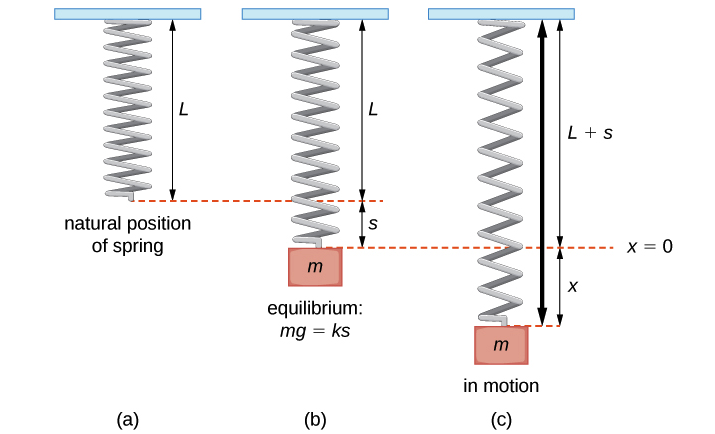
\includegraphics[scale=0.4]{phys232/Ch3-g-new-eqm} \caption{Gravity shifts the equilibrium position of a SHO by a distance $h$.}\label{ch3:fig-g-new-eqm-pos}
\end{figure}

Gravity only changes the equilibrium position of a SHO, without changing the amplitude, period, or frequency:
\begin{align*}
	F_\text{net} &= -F_\text{restoring} + F_g \\
	m\ddot{x} &= -kx + mg \\
	& = -k(x - \frac{mg}{k}) \\
	& = -k(x - h) \where h=\frac{mg}{k}
\end{align*}
Let $y=x-h$. This implies $\ddot{y} = \ddot{x}$. Therefore,
\begin{align*}
	&m\ddot{y} = -ky \\
	&m\ddot{y} + ky = 0  \Longrightarrow \text{still SHM!}
\end{align*}

We can interpret $h$ as the change in position that occurs when the mass is first hung or the floating object is first placed in a liquid and the system reaches \emph{static equilibrium} (see Figure \ref{ch3:fig-g-new-eqm-pos}).
\[ F_g = F_\text{restoring}\Longrightarrow mg = kh \Longrightarrow h = \frac{mg}{k} \]


\subsection{Systems analyzed using the conservation of energy}
\begin{center}
	\renewcommand{\arraystretch}{2.5}
	\begin{tabular}[t]{lll}
		\hline
		Type of system & Energy equation & $\omega^2$ \\ \hline
		Mass on spring &
			$\frac{1}{2}\mcol{m}\dot{x}^2 + \frac{1}{2}\kcol{k}x^2 = E $ &
			$\dfrac{\kcol{k}}{\mcol{m}}$
			\\
		Pendulum &
			$\frac{1}{2}\mcol{I}\dot{\theta}^2 + \frac{1}{2}\kcol{mgl}\theta^2 = E $ &
			$\dfrac{\kcol{mgl}}{\mcol{I}} = \dfrac{\kcol{mgl}}{\mcol{ml^2}}= \dfrac{\kcol{g}}{\mcol{l}}$ 
			\\
		\parbox{5.5cm}{Pendulum \footnotesize(with radius of gyration $k$, centre of mass at distance $h$ from point of suspension)}&
			$\frac{1}{2}\mcol{m(k^2+h^2)}\dot{\theta}^2 + \frac{1}{2}\kcol{mgh}\theta^2 = E $ &
			$\dfrac{\kcol{gh}}{\mcol{k^2+h^2}}$ 
			\\
		Water in a U-tube &
			$\frac{1}{2}\mcol{\rho Al}\dot{y} + \frac{1}{2}\kcol{(2g\rho A)}y^2 = E$ &
			$\dfrac{\kcol{2g}}{\mcol{l}}$ 
			\\
		Torsional oscillations &
			$\frac{1}{2}\mcol{I}\dot{\theta} + \frac{1}{2}\kcol{c}\theta^2 = E$ &
			$\dfrac{\kcol{c}}{\mcol{I}}$ 
			\\
		\parbox{5cm}{Massive springs \\\footnotesize{(with mass $M$)}} &
			$\frac{1}{2}\mcol{\left(m + \frac{1}{3}M \right)}\dot{x} + \frac{1}{2}\kcol{k}x^2 = E$ &
			$\dfrac{\kcol{k}}{\mcol{m + M/3}}$ 
			\\
		\hline
	\end{tabular}
	\renewcommand{\arraystretch}{1}
\end{center}


\section{Solving for the equation of motion of a harmonic oscillator}

\begin{proof}[Solving for the solution]
Rewrite \eqref{ch3:eq-NL} in terms of $k/m$:
\begin{align}
m\ddot{x} + kx &= 0 \notag\\
\ddot{x} + \frac{k}{m}x &= 0 \notag\\
\ddot{x} + \omega^2 x  &= 0 \label{ch3:eq-xdd}
\end{align}

\eqref{ch3:eq-xdd} implies $\ddot{x}$ is a multiple of $x$. This is a property of the exponential function, so write: 
\begin{equation}
	x=Ce^{pt} \label{ch3:eq-xCPT}
\end{equation}
where $p$ is a dimensional constant such that $pt$ is dimensionless, and $C$ is a coefficient.
%
\begin{align*}
\intertext{Sub \eqref{ch3:eq-xCPT} back into \eqref{ch3:eq-xdd}:}
\frac{d^2}{dt^2}(Ce^{pt})+\omega^2(Ce^{pt}) &= 0\\
p^2Ce^{pt}+\omega^2Ce^{pt}&=0 \\
Ce^{pt}(p^2+\omega^2) &=0 \\
\Longrightarrow p^2 + \omega^2 &= 0 \\
p^2 &= -\omega^2 \\
p &= \pm j\omega
\end{align*}

Because we have two possibilities for $p$, our solution to \eqref{ch3:eq-xdd} could have been written more generally as:
\[ x = C_1e^{j\omega t}+C_2e^{-j\omega t} \]


Geometrically, $x$ is the sum of two vectors: one with length $C_1$ rotating CCW and another with length $C_2$ going CW, both with the same angular displacement $\omega t$ (see Figure~\ref{ch3:fig-complex-sols}a).

In order to produce a harmonic oscillation along the $x$-axis, the $y$-components of the vectors must cancel. This is also the case when we have an initial phase angle $\alpha\neq 0$ (see Figure~\ref{ch3:fig-complex-sols}b).

\begin{figure}[h]
	\centering
	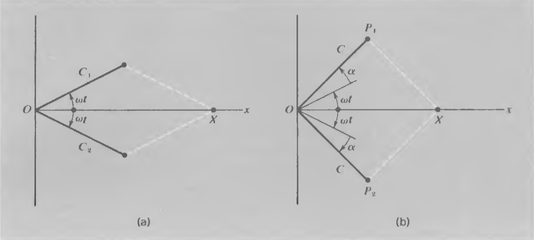
\includegraphics[scale=0.8]{phys232/Ch3-adding-complex-solutions.png} \caption{Superposition of complex solutions of \eqref{ch3:eq-xdd} with (a) $\alpha=0$ and (b) $\alpha\neq 0$. For $OX$ to be a harmonic oscillation, $C1=C2$.}\label{ch3:fig-complex-sols}
\end{figure}


For the $y$-components to cancel, we need $C_1=C_2$. Hence,
\begin{align*}
x
&=Ce^{j(\omega t +\alpha)} + Ce^{-j(\omega t +\alpha)} \\
&=C[\cos(\omega t + \alpha) + j\sin(\omega t + \alpha) + \cos(-(\omega t + \alpha)) + j\sin(-(\omega t + \alpha))] \\
&=C[\cos(\omega t + \alpha) + \cancel{j\sin(\omega t + \alpha)} + \cos(\omega t + \alpha) - \cancel{j\sin(\omega t + \alpha)}] \\
&= 2C\cos(\omega t + \alpha) \\
\therefore
x &= Acos(\omega t + \alpha) \where A=2C
\end{align*}

This is why, for SHM in general, we can assume solutions of the type:
\begin{equation}
	x=\Re(z) \where z=Acos(\omega t + \alpha)
\end{equation}
\end{proof}


\section{Elastic Wire \& Young's Modulus}

Apply a force $F_\text{app}$ to one end (e.g., by hanging a mass off it) and let the other end remain fixed. When the wire/rod is in \textit{static equilibrium}, let us define two quantities:

\[  \text{strain} = \frac{x}{l_0} \where\text{$x$ is the extension of the wire}  \]

\[ \text{stress} = \frac{F_\text{app}}{A} \where\text{$A$ is the cross-sectional area} \]

The ratio between these two quantities is a constant $Y$, which we call \textbf{Young's modulus of elasticity} for the material\footnote{... as long as the strain is small enough, such that the material is not permanently deformed when stretched.}:
\[\boxed{ Y = \frac{\text{stress}}{\text{strain}} = \text{const} } \]

Let us consider the force $F = -F_\text{app}$ exerted \emph{by} the rod \emph{on} another object. Hence,
\begin{align*}
	& -Y = \frac{F/A}{x/l_0} \\
	& \boxed{\therefore F = \kcol{\frac{-AY}{l_0}} x \label{ch3:eq-youngs-F}}
\end{align*}


Once a mass $m$ is hung on one end:
\[ \omega^2 = \sqrt{\frac{\kcol AY}{\mcol m \kcol{l_0}}} \]

We can rewrite this in terms of properties more easily measured at static equilibrium, such as $h$, the increase of length reached at static equilibrium after the mass is attached.
\[ \mcol{m}g=\kcol{\frac{AY}{l_0}} h \Longrightarrow \frac{ml_0}{AY}=\frac{h}{g} \]
\begin{equation}
\therefore \omega^2 = \frac{g}{h}  \label{ch3:eq-elastic-wire-result}
\end{equation} 

Remark: this result is similar to that for a simple pendulum (Equation~\ref{ch3:eq-simple-pendulum-result}).

\section{Floating Objects}

\begin{figure}[h]
	\centering
	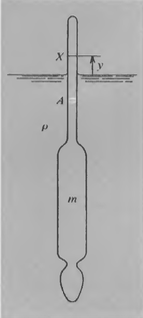
\includegraphics[scale=0.6]{phys232/Ch3-floating.png} \caption{Floating object at a vertical displacement of $y$ from its equilibrium position.}\label{ch3:fig-floating}
\end{figure}

Let the floating object (of mass $m$) have a constant cross-sectional area $A$ parallel to the liquid surface.

Recall:
\[ F_\text{buoyancy} = \text{weight of liquid displaced by the floating object} \]
\[ \boxed{F_b  = \kcol{g\rho A}y} \]

where...
\begin{itemize}
	\item $\rho$: density of the liquid
	\item $y$: vertical displacement of the object above equilibrium position
\end{itemize}


By Newton's Law:
\[ \mcol{m}\frac{d^2y}{dt^2} = -\kcol{g\rho A}y \]
\[ \therefore \omega^2 = \frac{\kcol{g\rho A}}{\mcol{m}} \]

We can, again, rewrite $\omega^2$ in terms of $h$, the change in equilibrium position when the object is placed in the liquid and reaches static eqm:
\[ \mcol{m}\cancel{g}=\kcol{\cancel{g}\rho A} h
\Longrightarrow
h = \frac{m}{\rho A} \]
\[ \therefore \omega^2 = \frac{g}{h} \]


This is analogous to the $\omega^2$ of an elastic wire, seen earlier in \eqref{ch3:eq-elastic-wire-result}. 


\section{The Pendulum}
\begin{figure}[h]
	\centering
	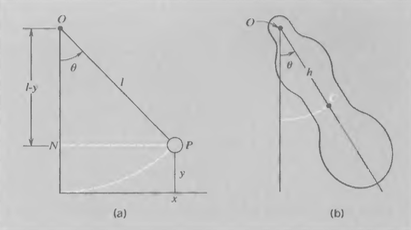
\includegraphics[scale=0.6]{phys232/Ch3-pendulum.png} \caption{(a) Simple pendulum; (b) pendulum of arbitrary shape with its centre of mass at $C$.}\label{ch3:fig-pendulum}
\end{figure}

Let $\theta$ represent the angular displacement of the pendulum. Assume small $\theta$ such that $y \ll x$. 


\subsection{Simple Pendulum}
By the Pythagorean Theorem (see Figure~\ref{ch3:fig-pendulum}):
\begin{align}
l^2 &= x^2 + (l-y)^2  \notag \\	
\cancel{l^2} &= x^2 + \cancel{l^2} - 2ly + y^2 \notag \\
x^2 &= 2ly - {y^2} \notag \\
x^2 &\approx 2ly  \notag \\
\Longrightarrow y &\approx \frac{x^2}{2l} \label{ch3:eq-pendulum-pythag}
\end{align}

In addition,
\begin{equation}
v^2=\left( \frac{dx}{dt} \right)^2 + \left(\frac{dy}{dt} \right)^2
\approx  \left( \frac{dx}{dt} \right)^2 \label{ch3:eq-pendulum-v2}
\end{equation}

By the Conservation of Energy and using the approximations \eqref{ch3:eq-pendulum-pythag} and  \eqref{ch3:eq-pendulum-v2}:
\begin{align}
\frac{1}{2} mv^2 + mgy &= E \notag \\
\frac{1}{2} \mcol{m} \left( \frac{dx}{dt} \right)^2 + \frac{1}{2} \kcol{\frac{mg}{l}} x^2 &= E  \label{ch3:eq-pendulum-E}
\end{align}


We can rewrite this result in terms of $\theta$. Substitute\footnote{Use the small angle approximation $\cos\theta \approx 1-\frac{\theta^2}{2}$, from Equation~\eqref{ch1:eq-small-angle-cos}}:
\begin{equation*}
v = l\left(\frac{d\theta}{dt}\right) \andd
y = l(1-\cos\theta) \approx \frac{1}{2}l\theta ^2
\end{equation*}

So, \eqref{ch3:eq-pendulum-E} becomes:
\begin{equation}
	\frac{1}{2} \mcol{ml^2} \left( \frac{d\theta}{dt} \right)^2 + \frac{1}{2} \kcol{mgl} \theta^2 = E \label{ch3:eq-pendulum-E-theta}
\end{equation}

Both \eqref{ch3:eq-pendulum-E} and \eqref{ch3:eq-pendulum-E-theta} imply that:
\begin{equation}
	\therefore \omega^2 = \frac{g}{l} \label{ch3:eq-simple-pendulum-result}
\end{equation}


\subsection{Pendulum of an Arbitrary Shape}
Let its center of mass $C$ be at a dist $h$ from the point of suspension $O$\footnote{This allows us to find the PE of the pendulum using the height of the CM.}, as shown in Figure~\ref{ch3:fig-pendulum}b.

\subsubsection{Using the moment of inertia w.r.t. the point of suspension}

Let $I$ represent the moment of inertia \emph{with respect to $O$}. Then:
\begin{equation*}
PE = \frac{1}{2} mgh\theta^2 \andd
KE = \frac{1}{2} I\left( \frac{d\theta}{dt} \right)^2
\end{equation*}

So,
\begin{equation} \frac{1}{2} \mcol{I}\left( \frac{d\theta}{dt} \right)^2 + \frac{1}{2} \kcol{mgh}\theta^2 = E \label{ch3:eq-pendulumEO}
\end{equation}

\subsubsection{Using the moment of inertia w.r.t. the centre of mass}
From the \emph{parallel axis theorem} -- at point $C$, we have:
\begin{align*}
	I_C &= I_\text{CM} + mh^2 \\
	&= mk^2 + mh^2
\end{align*}

where $k$ is the \emph{radius of gyration}. Thus,
\begin{align*}
	KE_C %&= \frac{1}{2} ( I_\text{CM} + mh^2 ) \left( \frac{d\theta}{dt} \right)^2 \\
	&= \frac{1}{2} m(k^2 + h^2 ) \left( \frac{d\theta}{dt} \right)^2
\end{align*}

Then, \eqref{ch3:eq-pendulumEO} becomes:
\[ \frac{1}{2} \mcol{m(k^2+h^2)} \left( \frac{d\theta}{dt} \right)^2  + \frac{1}{2} \kcol{mgh}\theta^2 = E \]

\begin{equation*}
	\therefore \omega^2 = \frac{\kcol{gh}}{\mcol{m(k^2+h^2)}}
\end{equation*}

This result is analogous to what we found for an elastic wire (Equation~\ref{ch3:eq-elastic-wire-result}).

\section{Liquid in a U-Tube}
Examine the vertical displacement $y$ of the liquid surface from equilibrium.

Let $l, A, \rho$ represent, respectively: total length of liquid column, cross sectional area, and liquid density.

Then, the total mass of the liquid is $m=\rho Al$. Assume all parts of the liquid move with speed $dy/dx$/

When liquid \textit{rises} a height of $y$ in one end, the liquid in the other end \textit{sinks} a height of $y$. This liquid displacement is associated with a change of potential energy of
\[ U = g\rho Ay^2 \]

By Conservation of Energy:
\[ \frac{1}{2}\rho Al \left( \frac{dy}{dt} \right)^2 + g\rho Ay^2 = E  \] 

Thus:
\begin{equation}
\omega^2 = \frac{2g}{l} \label{ch3:eq-utube-result}
\end{equation}

Again, the result for a U-tube \eqref{ch3:eq-utube-result} is comparable to that for an elastic wire \eqref{ch3:eq-elastic-wire-result}.

\section{Torsional Oscillations}
If the torque $M \propto$ angular displacement $\theta$ between two ends of an object,
\[ M=-c\theta \where\text{$c$ is the torsion constant of the system.} \]

Stored potential energy: \[ U= -\int M d\theta = \frac{1}{2} c\theta^2 \]

If one end has a moment of inertia $I$ and the inertia of the twisted system itself is negligible, then by energy conservation:
\[ \frac{1}{2}I\left( \frac{d\theta}{dt}\right)^2 + \frac{1}{2} c\theta^2 = E \]

Thus:
\begin{equation}
\omega^2 = \frac{c}{I} \text{ and } T = 2\pi\sqrt{\frac{I}{c}} \label{torsionalT}
\end{equation}

\subsection{Shear Modulus}
Apply a horizontal force $P$ to the board in a). Two of the sides change from rectangles to parallelograms. Define an \textbf{angle of shear, $\alpha$}:
\[ \alpha = \frac{x}{l} \]

Let $F=-P$ represent the force exerted \textit{by the sheared material} onto the board.

Define a \textbf{shear modulus} or \textbf{modulus of rigidity}, $n$:
\[ n = \frac{-F/A}{\alpha} \]
or
\begin{equation} \boxed{dF = -nA d\alpha = \frac{-nA}{l}dx} \label{shear_dF} \end{equation}

Notice that \eqref{shear_dF} for \textit{shear deformations} is analogous to \eqref{youngs_dF} and \eqref{ch3:eq-youngs-F} for \textit{longitudinal deformations}.

(Another modulus also exists: the \textbf{bulk modulus}, $K$, which describes the resistance of a material to changes in volume.)

\subsection{Restoring Torques}
Refer to the figure in b).

Two disks of radius $r$ on spindles are connected by two rectangular strips of material.

Twist one spindle through a small $\theta$; the end of each strip is moved transversely through a distance $r\theta$.

The angle of shear is thus: \[ \alpha = \frac{r\theta}{l} \]

Sub into \eqref{shear_dF} to find the restoring force tangential to the disk by each strip (if they have a cross-sectional area of $A$:
\[ F = -nA\frac{r\theta}{l} \]

There is a torque of magnitude $rF$ exerted about the axis of twist by each strip.

\subsubsection{Thin Walled Tube}
Refer to the figure in c).

Let the mean radius be $r$ and the wall thickness be $\Delta r$.

Consider it a whole collection of thin strips parallel to the axis of the cylinder, all contributing restoring torques about the axis.

So, when the tube is given a relative twist through $\theta$, the torque $\Delta M$ provided is:
\begin{align}
\Delta M &= -\frac{nAr^2\theta}{l}
\intertext{But here, $A=2\pi r \Delta r$:}
\Delta M &= -\frac{2\pi nr^3\Delta r}{l} \theta \label{thinTube_dM}
\end{align}

\subsubsection{Solid Tube}
To find the torque provided by a \textit{solid} tube or cylinder, integrate or sum the above in \eqref{thinTube_dM} to obtain:
\begin{equation} \boxed{M = -\frac{\pi nr^4}{2l} \theta} \end{equation}

\section{``The Spring of Air"}
Consider a closed piston-gas system, as pictured. Let $m$ represent the mass of the movable piston, and let $p$ represent the pressure of the gas inside the tube.

When the piston moves a distance of $y$ from equilibrium position, the pressure inside changes by $\Delta p$:
\[ F = A\Delta p \]

Calculate the pressure change, using \emph{Boyle's Law}:
\begin{align*}
pV &= \text{const} \\
p\Delta V + V\Delta p &= 0 \tag{a bit like the product rule for differentiation}
\end{align*}

But, $\Delta V = Ay \Longrightarrow V = Al$ \\
So: \[ \Delta p = -\frac{py}{l} \]
Thus: \begin{equation} \boxed{ F=-\frac{Ap}{l}y } \label{pistonF} \end{equation}

Compare \eqref{pistonF} with \eqref{ch3:eq-youngs-F} for stretching/compressing a solid rod. Here, the $p$ is analogous to $Y$.

\subsection{Bulk Modulus}
\begin{align}
K &= -\frac{dp}{dV/V} \notag \\
&= -V\frac{dp}{dV}
\end{align}

Remember that Boyle's law requires \emph{isothermal} (constant temperature) conditions. So, define: \begin{equation} K_{isothermal} = p \label{Kisothermal} \end{equation} 
 
When a gas is compressed, \textit{it becomes warmer} because of the work being done on it (although this effect was ignored when deriving the expression for a small change in pressure and for the restoring force).

$P \propto$ mean-squared molecular speed, so the heating results in a greater restoring force than otherwise, and the elastic modulus of the gas column is larger than the $p$ predicted by \eqref{Kisothermal}.

Under completely \textbf{adiabatic} conditions (closed system; no heat flow in/out of the gas):
\begin{equation} pV^\gamma \end{equation}

Becomes:
\begin{align}
\ln p + \gamma\ln V &= \text{const} \notag \\
\frac{1}{p}\frac{dp}{dV} + \frac{\gamma}{V} &= 0 \notag \\
K_{adiabatic} = -V \frac{dp}{dV} &= \gamma p \label{Kadiabatic}
\end{align}

Elasticity is enhanced under adiabatic conditions, and therefore the \textit{frequency} of vibrations is increased.

\section{Oscillations Involving Massive Springs}
Consider: a mass $m$ on a uniform spring of total mass $M$ and spring constant $k$.

Each point on the spring undergoes a displacement proportional to their distances from the fixed end (just like in static extension).

Let the relaxed length of the spring be $l$. Let the distance from the fixed end be $s$ $(0 \leq s \leq l)$. 

Consider an infinitesimal segment of the spring between $s$ and $s + ds$.

Its mass is: \[ dM = \frac{M}{l} ds \] 

Its displacement is \[ \frac{s}{l} x \]

Its kinetic energy is \[ dK = \frac{1}{2}\left( \frac{M}{l} ds \right) \left( \frac{s}{l} \frac{dx}{dt} \right)^2 = \frac{M}{2l^3} \left( \frac{dx}{dt} \right)^2 s^2 ds \]

Integrate, treating $dx/dt$ as a constant:
\begin{align*}
K_{spring} &= \frac{M}{2l^3} \left( \frac{dx}{dt} \right)^2  \int_0^{l} s^2 ds \\
&= \frac{1}{6}M\left(\frac{dx}{dt}\right)^2
\end{align*}

So, the energy-conservation statement for the whole system becomes:
\[ \frac{1}{2}m\left(\frac{dx}{dt}\right) + \frac{1}{6}M\left( \frac{dx}{dt}\right)^2 + \frac{1}{2}kx^2 = E \]
giving
\[ \omega^2 = \frac{k}{m + M/3} \]

This is the equivalent of taking a massless spring, and then adding a mass of $m + M/3$ to the end.


\section{The Decay of Free Oscillations}

\section{Large Damping}

%\chapter{Forced Vibrations \& Resonance}
%Cock, cock, teabag! 8=====|)

%\chapter{Free Vibrations}
\section{Damping}
Resistive forces, for small $v$: \[ F=-bv \]

Equation of motion:
\[ m\ddot{x} = -kx - b\dot{x} \]
\[ \ddot{x} + \gamma \dot{x} + {\omega_0}^2 x = 0 \]
where
\[ {\omega_0}^2 = k/m \text{ \& } \gamma = b/m \]

Solution:
\[ x = A e^{-\gamma t/2} \cos(\omega t + \alpha) \]
where
\[ \omega ^2 = \omega_0^2 - \frac{\gamma^2}{4} \]

Amplitude:
\[ A(t) = A_0 e^{-\gamma t/2} \]

Total energy:
\[ E(t) = \frac{1}{2}kA^2 = \frac{1}{2}kA_0^2 e^{-\gamma t} = E_0 e^{-\gamma t} \]

Quality value:
\[ Q = \frac{\omega_0}{\gamma} \]

\subsection{Very Large Damping}
\subsubsection{Overdamping ($ \omega_0 \ll \gamma/2 $)}
\[ x = A_1 e^{-(\gamma/2 + \beta)t} + A_2 e^{-(\gamma/2-\beta)t} \]
where \[ \beta = \left(\frac{\gamma^2}{4}-\omega_0^2 \right)^{1/2} \]

\subsubsection{Critical Damping ($ \omega_0 = \gamma/2 $)}
\[ x = (A + Bt) e^{\gamma t/2}\]

\chapter{Forced Vibrations \& Resonance}
\section{Forced Oscillations w/ Damping}
Driving force:
\[ F(t) = F_0 \cos(\omega t) \]

Two stages:
\begin{enumerate}
\item \textbf{Transient state}: original system's ''natural" motion slowly damping out; driving force beginning to take over
\item \textbf{Steady state}: system oscillates at the \emph{driving force's frequency}, $\omega$
\end{enumerate}

\subsubsection{Steady State}

Equation of motion:
\[ m\ddot{x} = -kx - b\dot{x} + F_0 \cos(\omega t) \]
\[ \ddot{x} + \gamma\dot{x} + \omega_0^2 = F_0 \cos(\omega t) \]

Results: 
\[ x = A \cos (\omega t - \delta) \]
\[ A(\omega) = \frac{F_0/m}{[(\omega_0^2 - \omega^2)^2 + (\gamma\omega)^2]^{1/2}} \]
\[ \tan \delta (\omega) = \frac{\gamma\omega}{\omega_0^2 - \omega^2}\]

Independent of adjustable initial starting conditions!

\subsubsection{Transient Effects}
For $t<0$, let the object be at rest (i.e. it only starts moving at $t=0$).
\begin{align*}
x &= steady + transient \\
x &= A \cos (\omega t - \delta) + B e^{-\gamma t/2} \cos(\omega' + \beta)
\end{align*}

The transient part (system's ''natural" motion) dies out over time due to damping; after then, the steady state takes over. 

Transient part of the equation accounts for adjustable initial conditions!

A \emph{beat pattern} may be produced during this stage if $\omega'$ (system's freq w/ damping) and $\omega$ are similar.

\section{Power}
Power required to keep a driven oscillator going at the same amplitude:
\[ P = \frac{dW}{dt} = F\frac{dx}{dt} = Fv \]

\chapter{Coupled Oscillators \& Normal Modes}

\end{document}